\documentclass[12pt,letterpaper]{article}\usepackage{graphicx, color}
%% maxwidth is the original width if it is less than linewidth
%% otherwise use linewidth (to make sure the graphics do not exceed the margin)
\makeatletter
\def\maxwidth{ %
  \ifdim\Gin@nat@width>\linewidth
    \linewidth
  \else
    \Gin@nat@width
  \fi
}
\makeatother

\IfFileExists{upquote.sty}{\usepackage{upquote}}{}
\definecolor{fgcolor}{rgb}{0.2, 0.2, 0.2}
\newcommand{\hlnumber}[1]{\textcolor[rgb]{0,0,0}{#1}}%
\newcommand{\hlfunctioncall}[1]{\textcolor[rgb]{0.501960784313725,0,0.329411764705882}{\textbf{#1}}}%
\newcommand{\hlstring}[1]{\textcolor[rgb]{0.6,0.6,1}{#1}}%
\newcommand{\hlkeyword}[1]{\textcolor[rgb]{0,0,0}{\textbf{#1}}}%
\newcommand{\hlargument}[1]{\textcolor[rgb]{0.690196078431373,0.250980392156863,0.0196078431372549}{#1}}%
\newcommand{\hlcomment}[1]{\textcolor[rgb]{0.180392156862745,0.6,0.341176470588235}{#1}}%
\newcommand{\hlroxygencomment}[1]{\textcolor[rgb]{0.43921568627451,0.47843137254902,0.701960784313725}{#1}}%
\newcommand{\hlformalargs}[1]{\textcolor[rgb]{0.690196078431373,0.250980392156863,0.0196078431372549}{#1}}%
\newcommand{\hleqformalargs}[1]{\textcolor[rgb]{0.690196078431373,0.250980392156863,0.0196078431372549}{#1}}%
\newcommand{\hlassignement}[1]{\textcolor[rgb]{0,0,0}{\textbf{#1}}}%
\newcommand{\hlpackage}[1]{\textcolor[rgb]{0.588235294117647,0.709803921568627,0.145098039215686}{#1}}%
\newcommand{\hlslot}[1]{\textit{#1}}%
\newcommand{\hlsymbol}[1]{\textcolor[rgb]{0,0,0}{#1}}%
\newcommand{\hlprompt}[1]{\textcolor[rgb]{0.2,0.2,0.2}{#1}}%

\usepackage{framed}
\makeatletter
\newenvironment{kframe}{%
 \def\at@end@of@kframe{}%
 \ifinner\ifhmode%
  \def\at@end@of@kframe{\end{minipage}}%
  \begin{minipage}{\columnwidth}%
 \fi\fi%
 \def\FrameCommand##1{\hskip\@totalleftmargin \hskip-\fboxsep
 \colorbox{shadecolor}{##1}\hskip-\fboxsep
     % There is no \\@totalrightmargin, so:
     \hskip-\linewidth \hskip-\@totalleftmargin \hskip\columnwidth}%
 \MakeFramed {\advance\hsize-\width
   \@totalleftmargin\z@ \linewidth\hsize
   \@setminipage}}%
 {\par\unskip\endMakeFramed%
 \at@end@of@kframe}
\makeatother

\definecolor{shadecolor}{rgb}{.97, .97, .97}
\definecolor{messagecolor}{rgb}{0, 0, 0}
\definecolor{warningcolor}{rgb}{1, 0, 1}
\definecolor{errorcolor}{rgb}{1, 0, 0}
\newenvironment{knitrout}{}{} % an empty environment to be redefined in TeX

\usepackage{alltt}
\topmargin 0.0in
\oddsidemargin 0.0in
\textwidth 6.5in
\textheight 9.0in
\headheight 0.0in
\headsep 0.0in

\newcommand{\balpha}{\mbox{\boldmath $\alpha$}}
\newcommand{\bxi}{\mbox{\boldmath $\xi$}}
\newcommand{\bneta}{\mbox{\boldmath $\eta$}}
\newcommand{\btau}{\mbox{\boldmath $\tau$}}
\newcommand{\bSigmaz}{\mbox{\boldmath $\hat{\Sigma}_z$}}
\newcommand{\bthetaz}{\mbox{\boldmath $\hat{\theta}_z$}}
\newcommand{\bgamma}{\mbox{\boldmath $\gamma$}}
\newcommand{\bGamma}{\mbox{\boldmath $\Gamma$}}
\newcommand{\bSigma}{\mbox{\boldmath $\Sigma$}}
\newcommand{\bTheta}{\mbox{\boldmath $\Theta$}}
\newcommand{\bbeta}{\mbox{\boldmath $\beta$}}
\newcommand{\btheta}{\mbox{\boldmath $\theta$}}
\newcommand{\beps}{\mbox{\boldmath $\epsilon$}}
\newcommand{\bphi}{\mbox{\boldmath $\phi$}}
\newcommand{\bmu}{\mbox{\boldmath $\mu$}}
\newcommand{\xpx}{\mathbf{X}^\prime \mathbf{X}}
\newcommand{\xpxinv}{(\mathbf{X}^\prime \mathbf{X})^{-1}}
\newcommand{\bY}{\mathbf{Y}}
\newcommand{\bX}{\mathbf{X}}
\newcommand{\bI}{\mathbf{I}}
\newcommand{\by}{\mathbf{y}}
\newcommand{\ba}{\mathbf{a}}
\newcommand{\bb}{\mathbf{b}}
\newcommand{\bC}{\mathbf{C}}
\newcommand{\Exp}{\mathbb{E}}
\newcommand{\eps}{\epsilon}
\newcommand{\kron}{\otimes}
\newcommand{\barr}{\begin{array}}
\newcommand{\earr}{\end{array}}
\newcommand{\bne}{\begin{equation}}
\newcommand{\ene}{\end{equation}}
\newcommand{\bea}{\begin{eqnarray}}
\newcommand{\eea}{\end{eqnarray}}
\newcommand{\bean}{\begin{eqnarray*}}
\newcommand{\eean}{\end{eqnarray*}}
\newcommand{\bit}{\begin{itemize}}
\newcommand{\eit}{\end{itemize}}
\newcommand{\benum}{\begin{enumerate}}
\newcommand{\eenum}{\end{enumerate}}
\title{Code for suitability functions and graphs}
\author{Dominic LaRoche}

\begin{document}
\maketitle





\section{Dr. Dave Ellis}
Shrub forb and grass diversity as described by Dr. Dave Ellis all follow a Gamma CDF.\\ 
\subsection{Shrub, Forb, and Grass Diversity}
\begin{center}
\begin{tabular}{p{1.5}cc}
$Description 
description 
description$ & $Equation
equation$ & \begin{figure}
\begin{knitrout}
\definecolor{shadecolor}{rgb}{0.969, 0.969, 0.969}\color{fgcolor}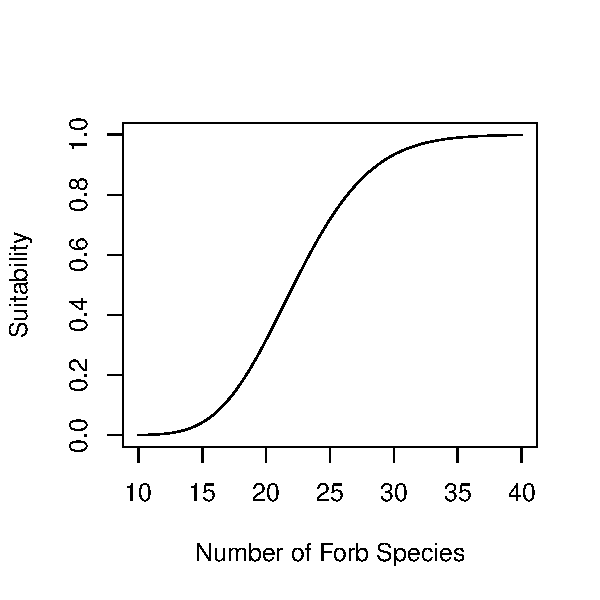
\includegraphics[width=\maxwidth]{figure/Ellis_Forb_diversity} 
\end{knitrout}

\end{figure}\\
Description & Equation &
\begin{knitrout}
\definecolor{shadecolor}{rgb}{0.969, 0.969, 0.969}\color{fgcolor}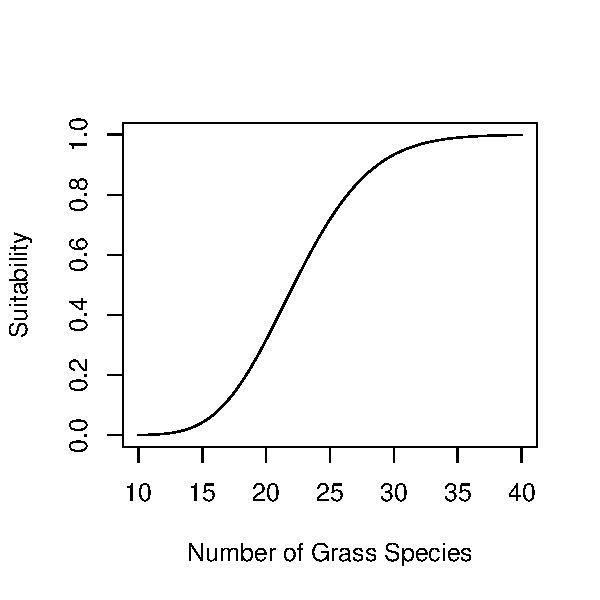
\includegraphics[width=\maxwidth]{figure/Ellis_Grass_diversity} 
\end{knitrout}

\\
Description & Equation &
\begin{knitrout}
\definecolor{shadecolor}{rgb}{0.969, 0.969, 0.969}\color{fgcolor}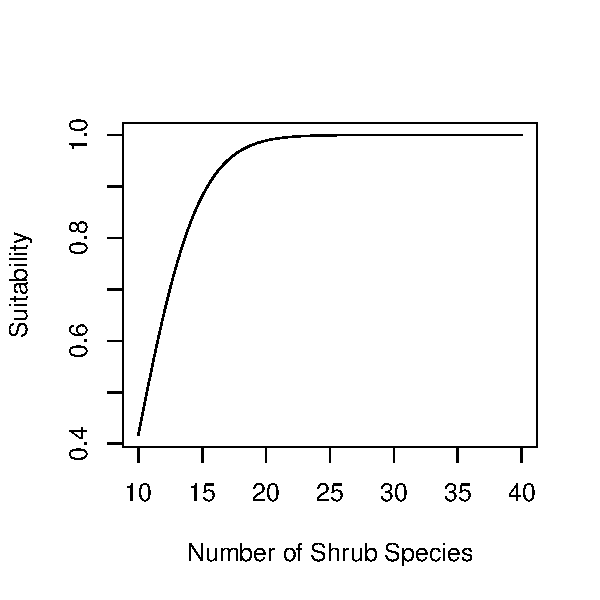
\includegraphics[width=\maxwidth]{figure/Ellis_Shrub_diversity} 
\end{knitrout}

\end{tabular}\\
\end{center}
\subsection{Forb Height}
The optimal forb height, as described by Dr. Ellis, is a 3 part function.

\begin{knitrout}
\definecolor{shadecolor}{rgb}{0.969, 0.969, 0.969}\color{fgcolor}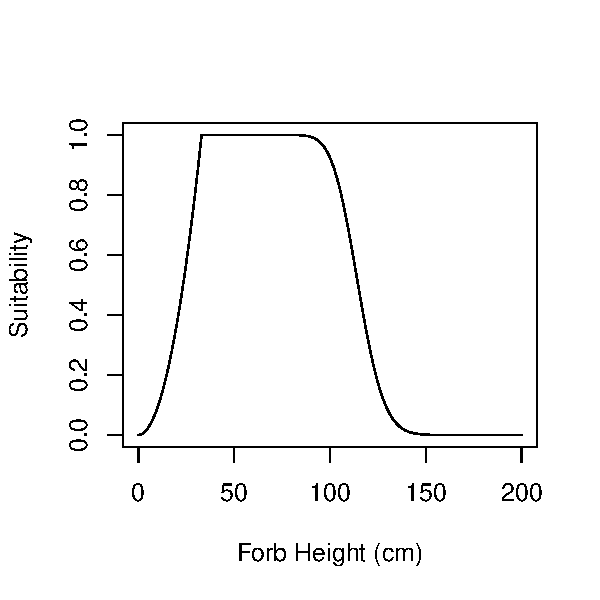
\includegraphics[width=\maxwidth]{figure/Ellis_Forb_Height} 
\end{knitrout}

\subsection{Shrub Height}
\begin{knitrout}
\definecolor{shadecolor}{rgb}{0.969, 0.969, 0.969}\color{fgcolor}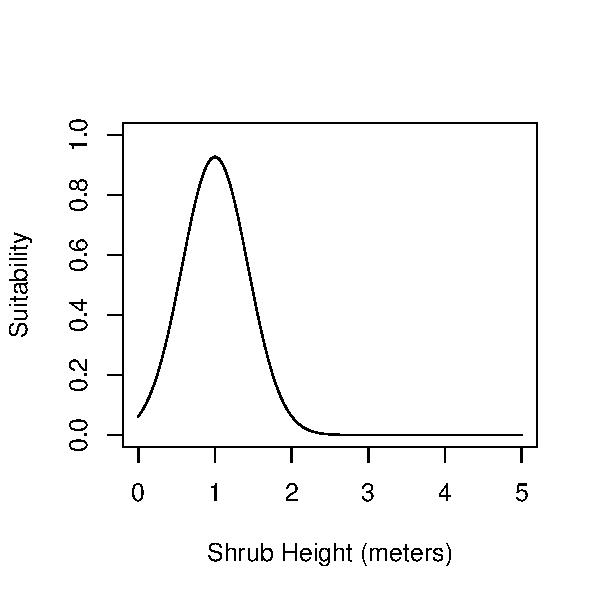
\includegraphics[width=\maxwidth]{figure/Ellis_Shrub_Height} 
\end{knitrout}

\subsection{Grass Cover}
\begin{knitrout}
\definecolor{shadecolor}{rgb}{0.969, 0.969, 0.969}\color{fgcolor}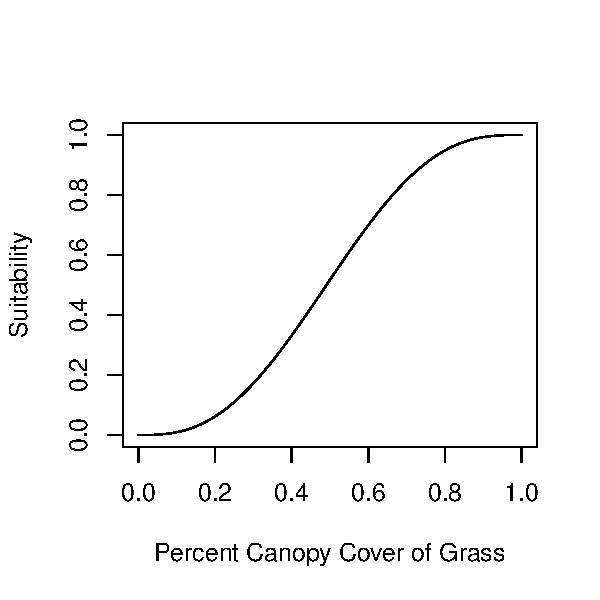
\includegraphics[width=\maxwidth]{figure/Ellis_Grass_Cover1} 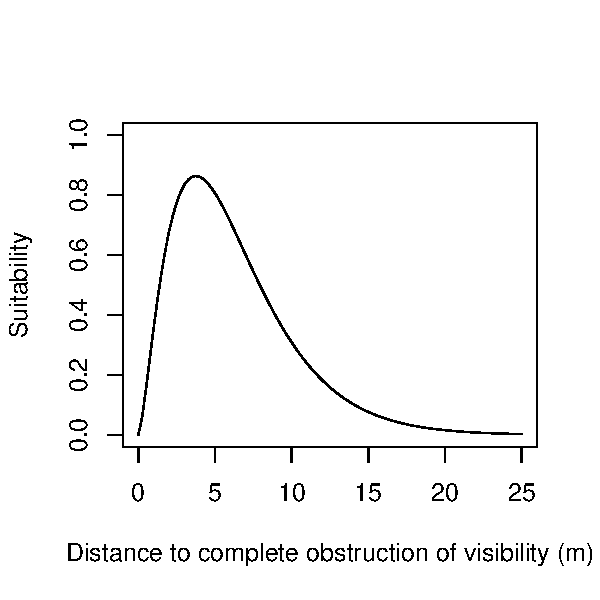
\includegraphics[width=\maxwidth]{figure/Ellis_Grass_Cover2} 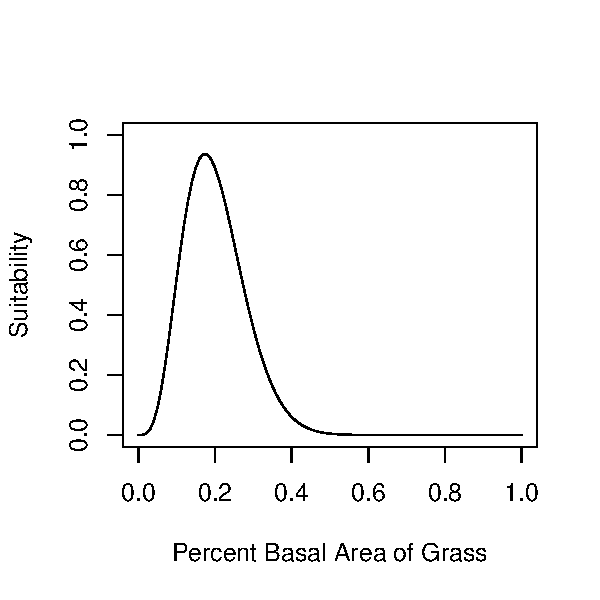
\includegraphics[width=\maxwidth]{figure/Ellis_Grass_Cover3} 
\end{knitrout}

\subsection{Tree Cover}
\begin{knitrout}
\definecolor{shadecolor}{rgb}{0.969, 0.969, 0.969}\color{fgcolor}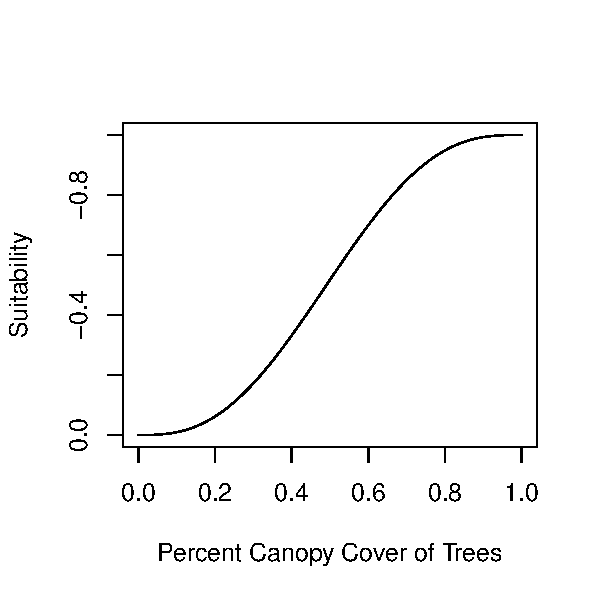
\includegraphics[width=\maxwidth]{figure/Ellis_Tree_Cover} 
\end{knitrout}

\subsection{Grass Height}
\begin{knitrout}
\definecolor{shadecolor}{rgb}{0.969, 0.969, 0.969}\color{fgcolor}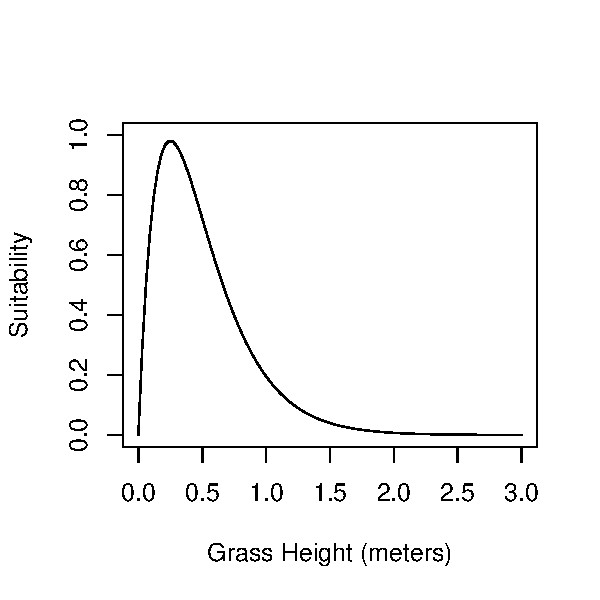
\includegraphics[width=\maxwidth]{figure/Ellis_Grass_Height} 
\end{knitrout}

\subsection{Structural Diversity}
\begin{knitrout}
\definecolor{shadecolor}{rgb}{0.969, 0.969, 0.969}\color{fgcolor}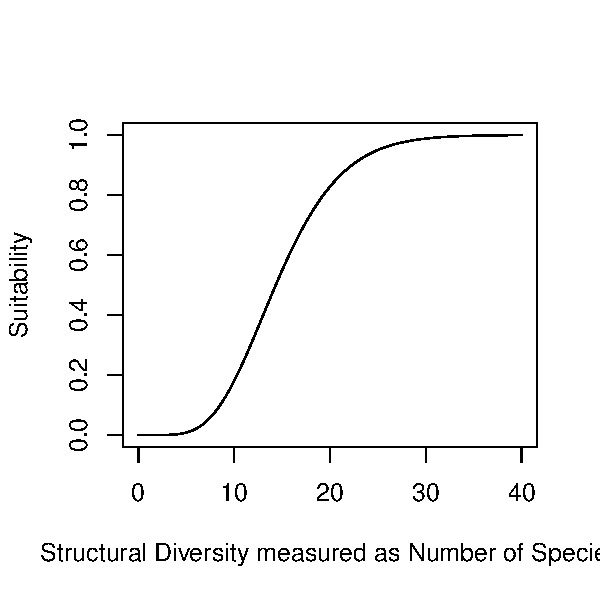
\includegraphics[width=\maxwidth]{figure/Ellis_Structural_Diversity} 
\end{knitrout}

\subsection{Total Cover}
\begin{knitrout}
\definecolor{shadecolor}{rgb}{0.969, 0.969, 0.969}\color{fgcolor}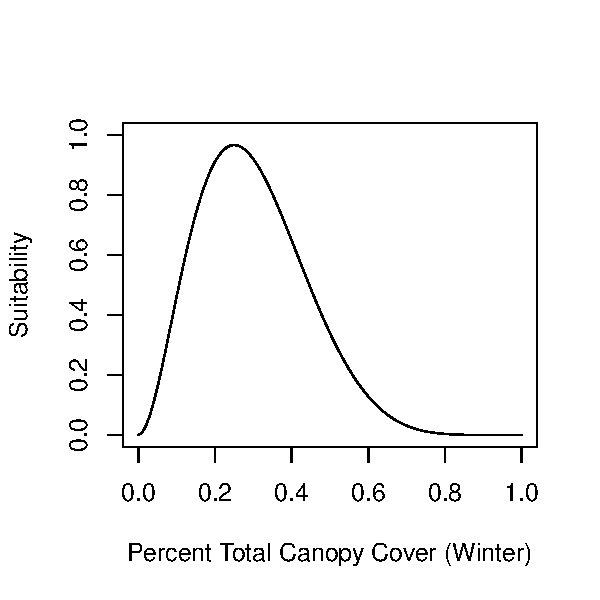
\includegraphics[width=\maxwidth]{figure/Ellis_Total_Cover1} 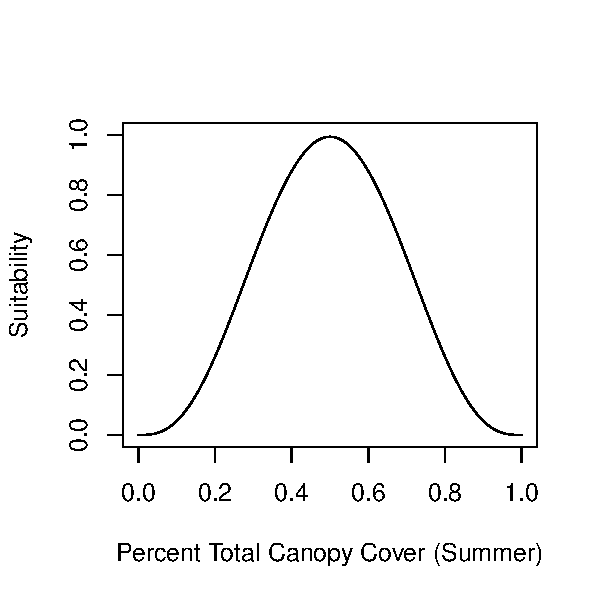
\includegraphics[width=\maxwidth]{figure/Ellis_Total_Cover2} 
\end{knitrout}

\section{John Goodwin}
\subsection{Forb Diversity}
\subsubsection{with gamma}
\begin{knitrout}
\definecolor{shadecolor}{rgb}{0.969, 0.969, 0.969}\color{fgcolor}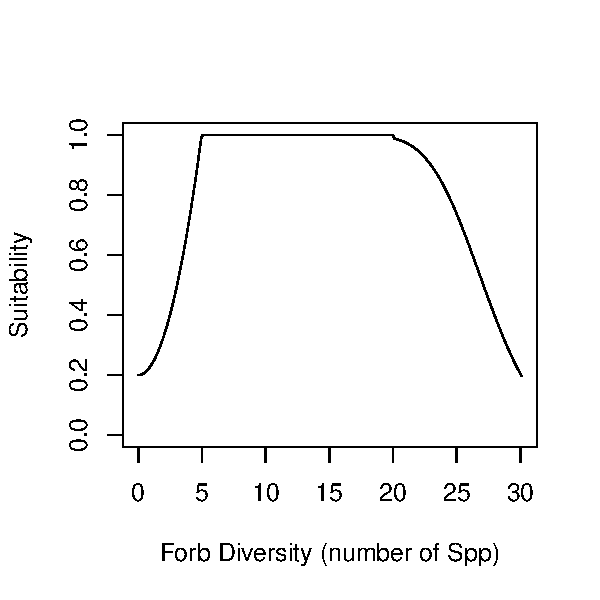
\includegraphics[width=\maxwidth]{figure/Goodwin_Forb_Diversity} 
\end{knitrout}


\\subsubsection{simple quadratic}
\begin{knitrout}
\definecolor{shadecolor}{rgb}{0.969, 0.969, 0.969}\color{fgcolor}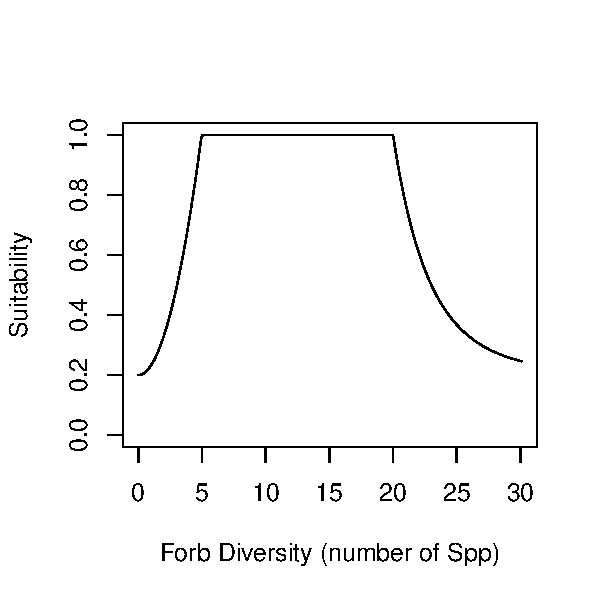
\includegraphics[width=\maxwidth]{figure/Goodwin_Forb_Diversity_alt} 
\end{knitrout}

\subsection{Forb Cover}
\subsubsection{Arizona}
\begin{knitrout}
\definecolor{shadecolor}{rgb}{0.969, 0.969, 0.969}\color{fgcolor}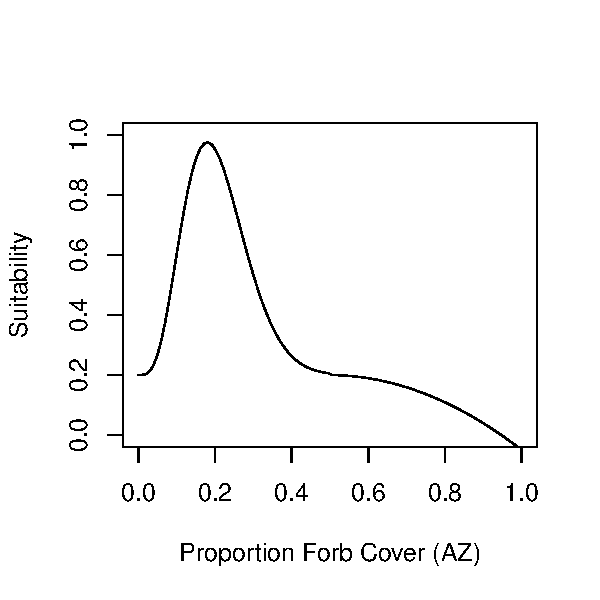
\includegraphics[width=\maxwidth]{figure/Goodwin_Forb_Cover_AZ} 
\end{knitrout}

\subsubsection{Mexico}
\begin{knitrout}
\definecolor{shadecolor}{rgb}{0.969, 0.969, 0.969}\color{fgcolor}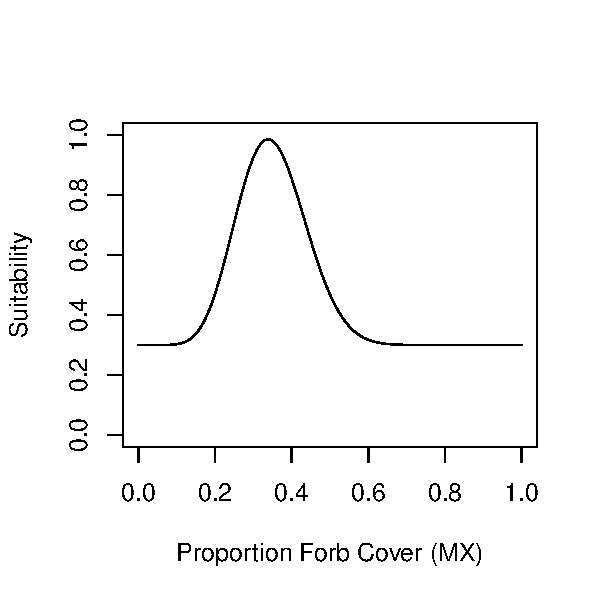
\includegraphics[width=\maxwidth]{figure/Goodwin_Forb_Cover_MX} 
\end{knitrout}

\subsection{Shrub Cover}
\subsubsection{Arizona}
\begin{knitrout}
\definecolor{shadecolor}{rgb}{0.969, 0.969, 0.969}\color{fgcolor}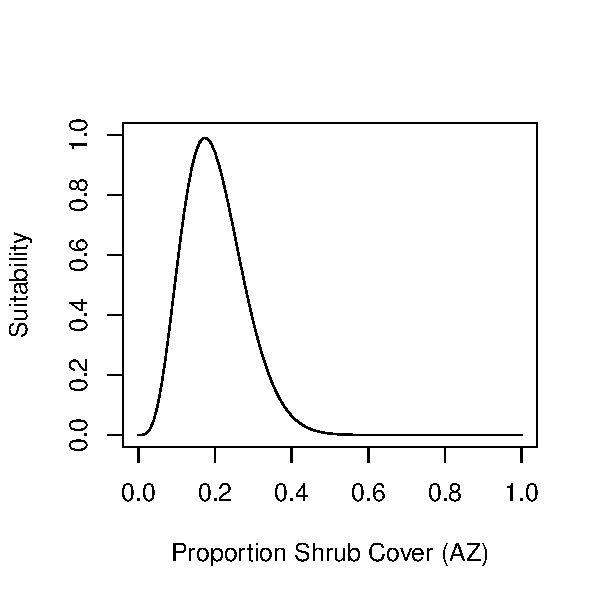
\includegraphics[width=\maxwidth]{figure/Goodwin_Shrub_Cover_AZ} 
\end{knitrout}

\subsubsection{Mexico}
\begin{knitrout}
\definecolor{shadecolor}{rgb}{0.969, 0.969, 0.969}\color{fgcolor}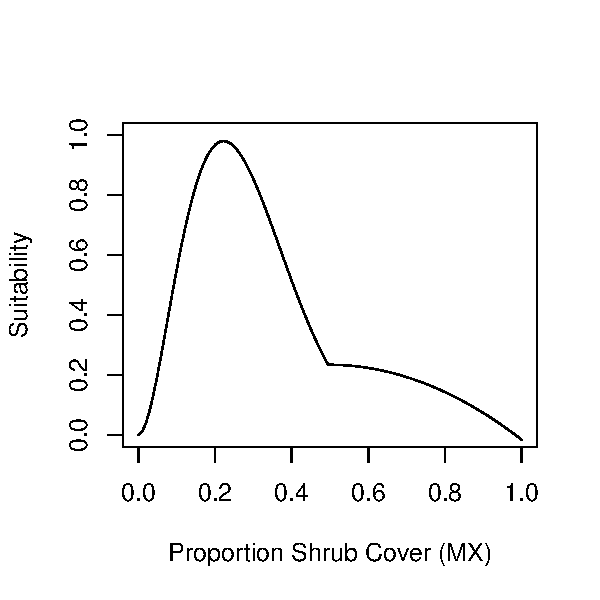
\includegraphics[width=\maxwidth]{figure/Goodwin_Shrub_Cover_MX} 
\end{knitrout}

\subsection{Grass Diversity}
\subsubsection{Mexico}
\begin{knitrout}
\definecolor{shadecolor}{rgb}{0.969, 0.969, 0.969}\color{fgcolor}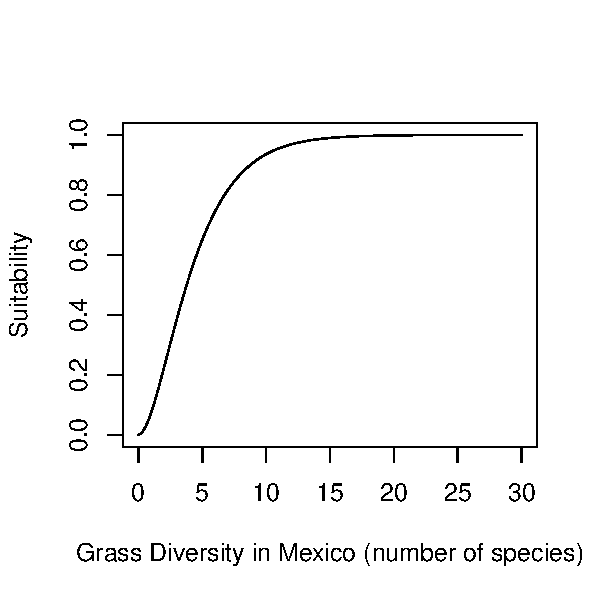
\includegraphics[width=\maxwidth]{figure/Goodwin_Grass-Diversity_MX} 
\end{knitrout}

\subsubsection{Arizona}
\begin{knitrout}
\definecolor{shadecolor}{rgb}{0.969, 0.969, 0.969}\color{fgcolor}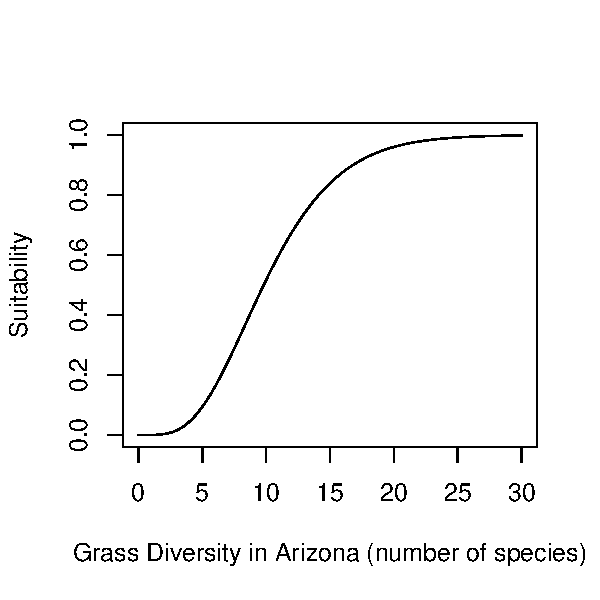
\includegraphics[width=\maxwidth]{figure/Goodwin_Grass-Diversity_AZ} 
\end{knitrout}

\subsection{Grass Cover}
\subsubsection{Mexico}
\begin{knitrout}
\definecolor{shadecolor}{rgb}{0.969, 0.969, 0.969}\color{fgcolor}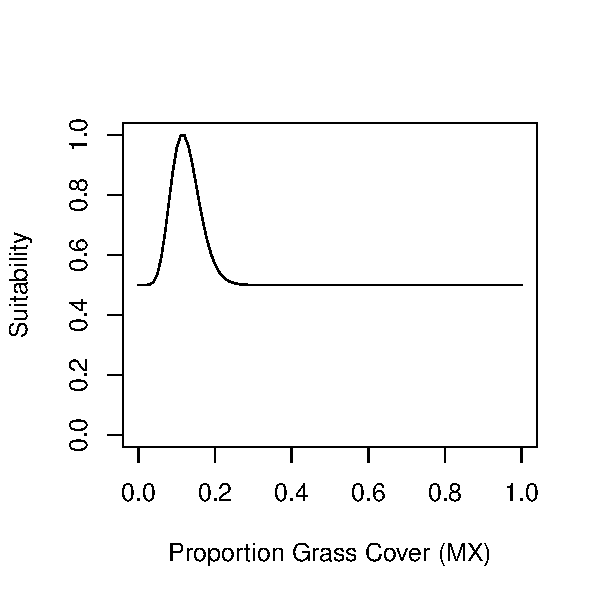
\includegraphics[width=\maxwidth]{figure/Goodwin_Grass_Cover_MX} 
\end{knitrout}

\subsubsection{Arizona}
\begin{knitrout}
\definecolor{shadecolor}{rgb}{0.969, 0.969, 0.969}\color{fgcolor}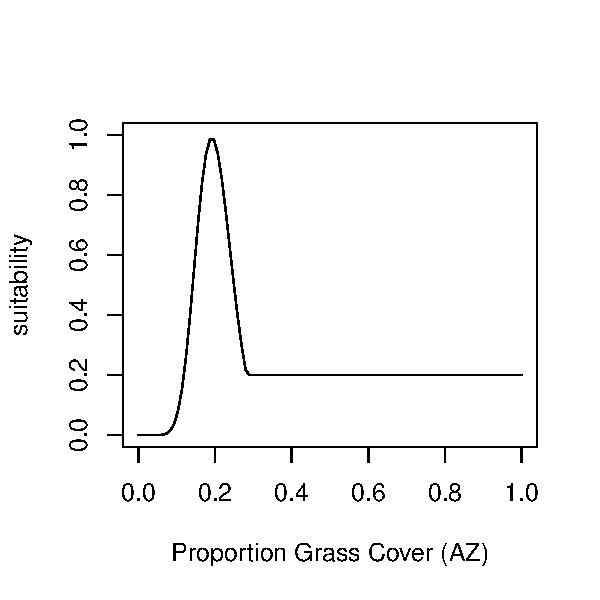
\includegraphics[width=\maxwidth]{figure/Goodwin_Grass_Cover_AZ} 
\end{knitrout}

\subsection{Tree Cover}
\subsubsection{Mexico}
\begin{knitrout}
\definecolor{shadecolor}{rgb}{0.969, 0.969, 0.969}\color{fgcolor}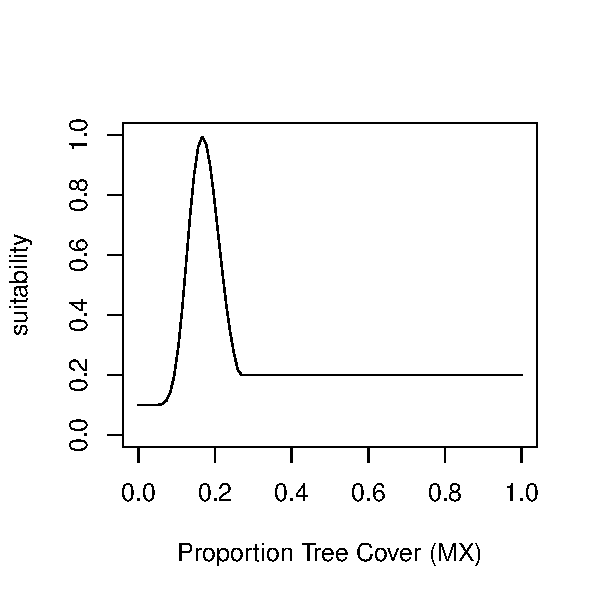
\includegraphics[width=\maxwidth]{figure/Goodwin_Tree_Cover_MX} 
\end{knitrout}

\subsubsection{Arizona}
\begin{knitrout}
\definecolor{shadecolor}{rgb}{0.969, 0.969, 0.969}\color{fgcolor}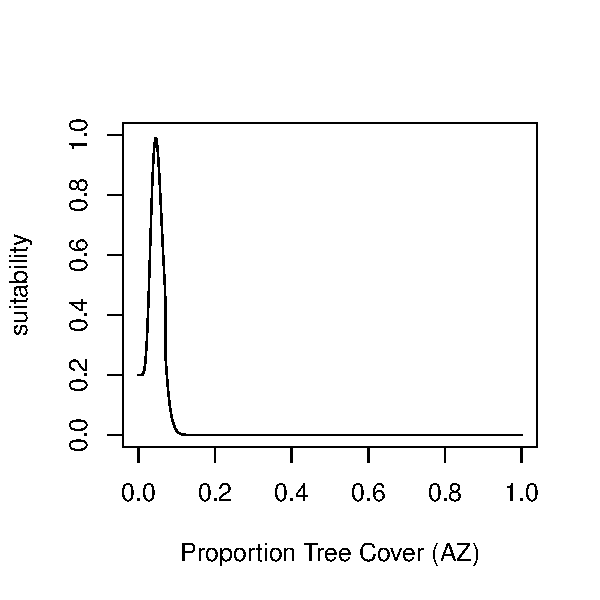
\includegraphics[width=\maxwidth]{figure/Goodwin_Tree_Cover_AZ} 
\end{knitrout}

\section{Sally Gall and Dan Cohan}
\subsection{Forb Diveristy}
\begin{knitrout}
\definecolor{shadecolor}{rgb}{0.969, 0.969, 0.969}\color{fgcolor}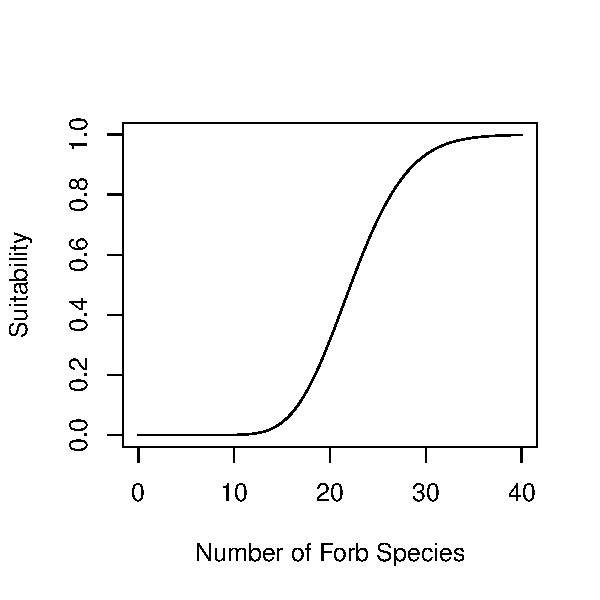
\includegraphics[width=\maxwidth]{figure/Sally-Dan_Forb_Diversity} 
\end{knitrout}

\subsection{Forb Height}
\subsubsection{Spring}
\begin{knitrout}
\definecolor{shadecolor}{rgb}{0.969, 0.969, 0.969}\color{fgcolor}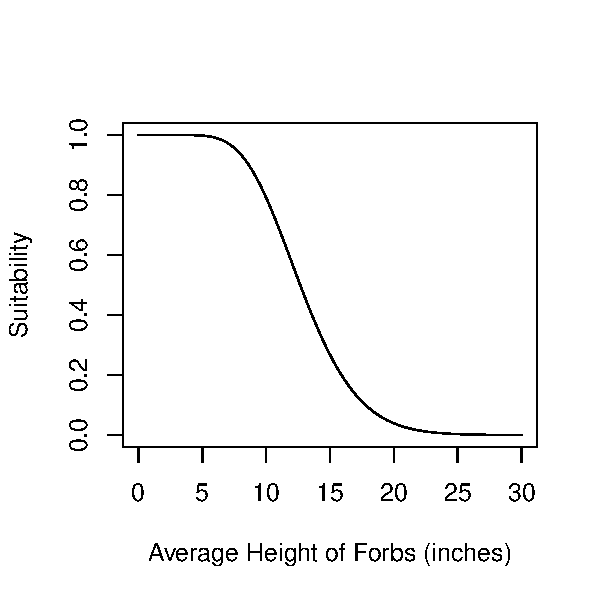
\includegraphics[width=\maxwidth]{figure/Sally-Dan_Forb_Height_spring} 
\end{knitrout}

\subsubsection{Fall}
\begin{knitrout}
\definecolor{shadecolor}{rgb}{0.969, 0.969, 0.969}\color{fgcolor}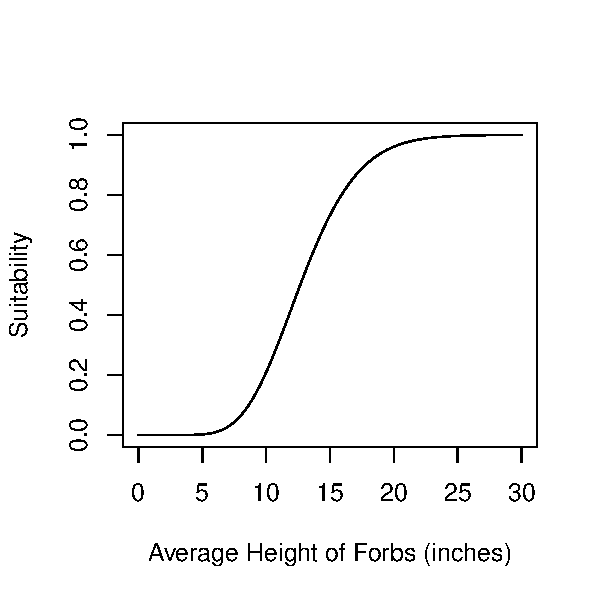
\includegraphics[width=\maxwidth]{figure/Sally-Dan_Forb_Height_fall} 
\end{knitrout}

\subsection{Forb Cover}
\subsubsection{Fall}
\begin{knitrout}
\definecolor{shadecolor}{rgb}{0.969, 0.969, 0.969}\color{fgcolor}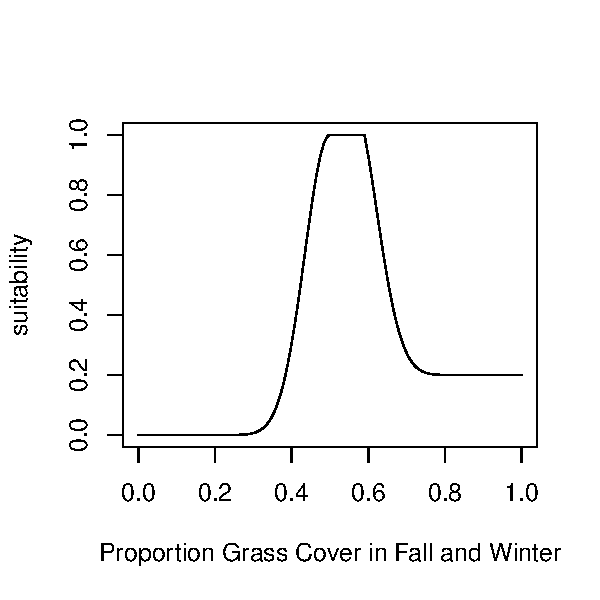
\includegraphics[width=\maxwidth]{figure/Sally-Dan_Forb_Cover_Fall} 
\end{knitrout}

\subsubsection{Spring}
\begin{knitrout}
\definecolor{shadecolor}{rgb}{0.969, 0.969, 0.969}\color{fgcolor}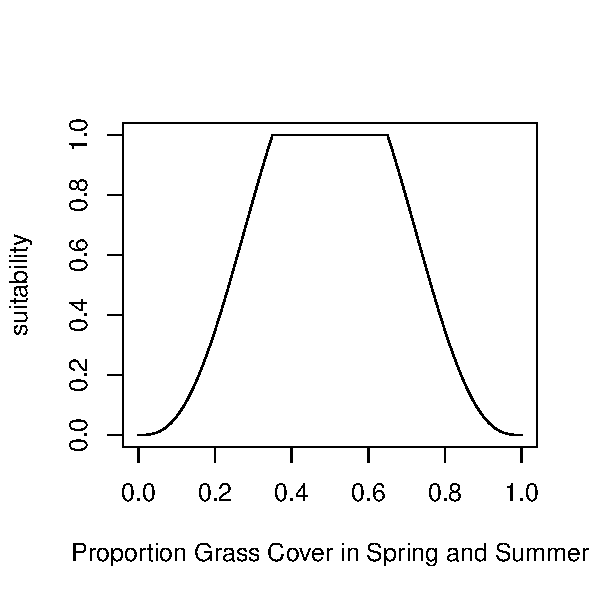
\includegraphics[width=\maxwidth]{figure/Sally-Dan_Forb_Cover_spring} 
\end{knitrout}

\subsection{Shrub Cover}
\subsubsection{Dan Cohan}
\begin{knitrout}
\definecolor{shadecolor}{rgb}{0.969, 0.969, 0.969}\color{fgcolor}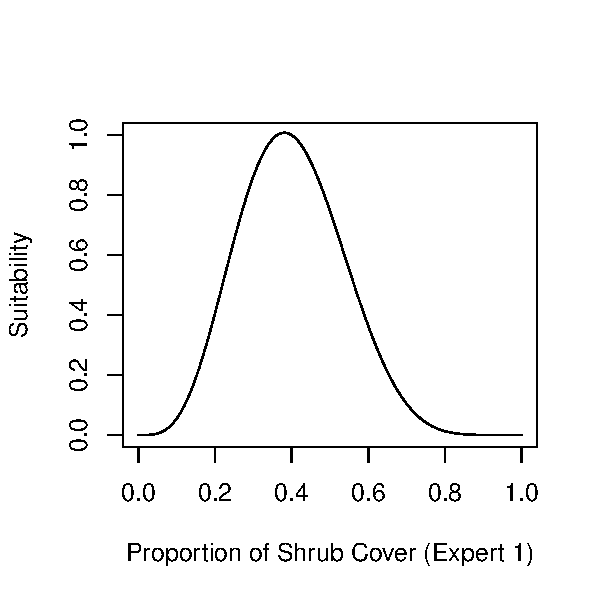
\includegraphics[width=\maxwidth]{figure/Dan_Shrub_Cover} 
\end{knitrout}

\subsubsection{Sally Gall}
\begin{knitrout}
\definecolor{shadecolor}{rgb}{0.969, 0.969, 0.969}\color{fgcolor}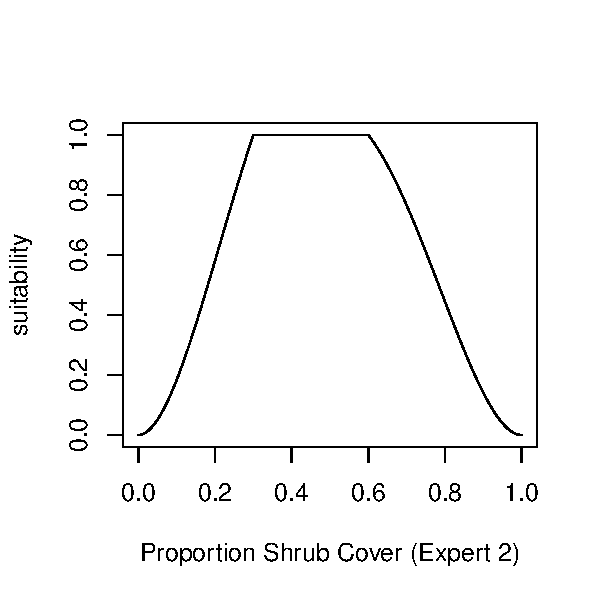
\includegraphics[width=\maxwidth]{figure/Sally_Shrub_Cover} 
\end{knitrout}

\subsection{Shrub Height}
\begin{knitrout}
\definecolor{shadecolor}{rgb}{0.969, 0.969, 0.969}\color{fgcolor}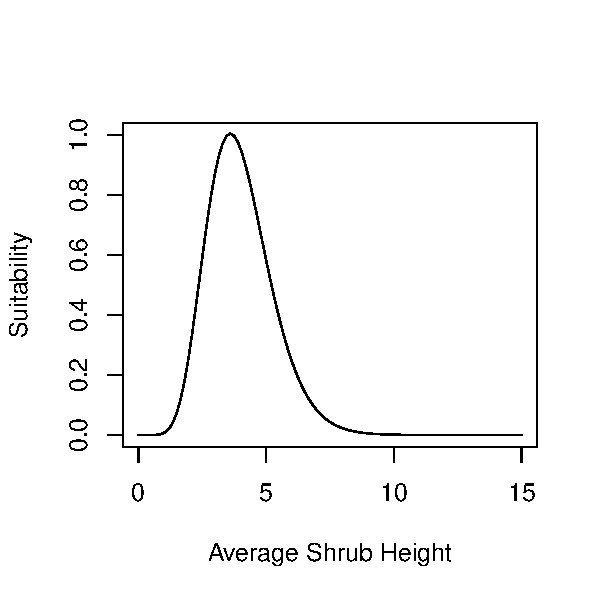
\includegraphics[width=\maxwidth]{figure/Sally-Dan_Shrub_Height} 
\end{knitrout}

\subsection{Grass Diversity}
\subsubsection{Perrenial}
\begin{knitrout}
\definecolor{shadecolor}{rgb}{0.969, 0.969, 0.969}\color{fgcolor}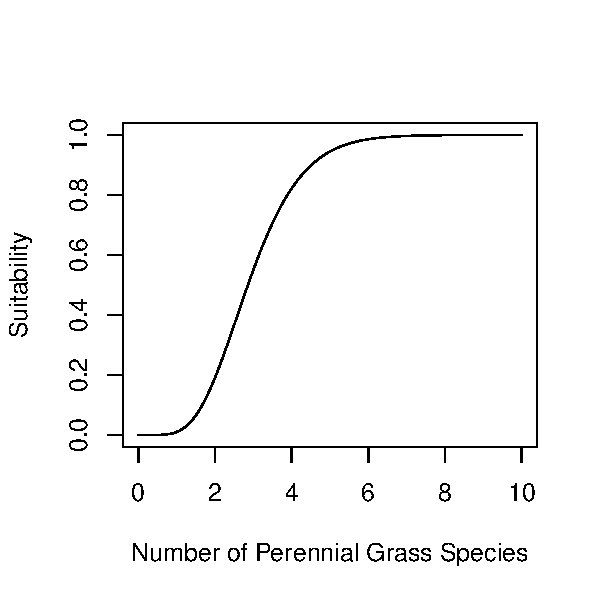
\includegraphics[width=\maxwidth]{figure/Sally-Dan_Grass_Diversity_p} 
\end{knitrout}

\subsubsection{Annual}
\begin{knitrout}
\definecolor{shadecolor}{rgb}{0.969, 0.969, 0.969}\color{fgcolor}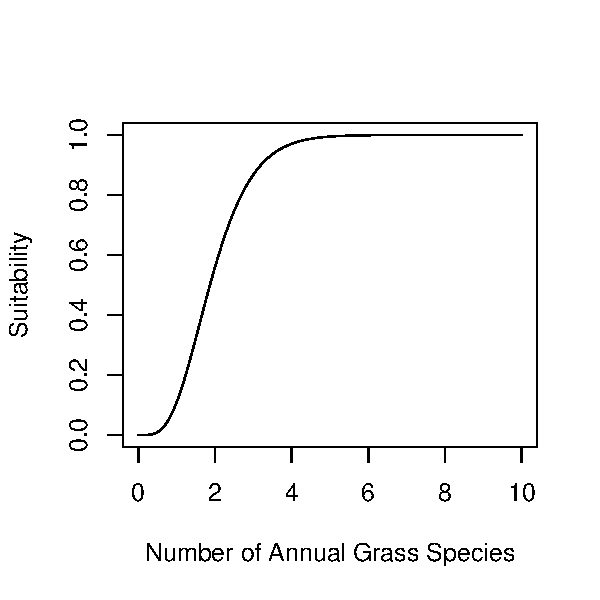
\includegraphics[width=\maxwidth]{figure/Sally-Dan_Grass_Diversity_a} 
\end{knitrout}

\subsection{Grass Cover}
\subsubsection{Perrenial}
\begin{knitrout}
\definecolor{shadecolor}{rgb}{0.969, 0.969, 0.969}\color{fgcolor}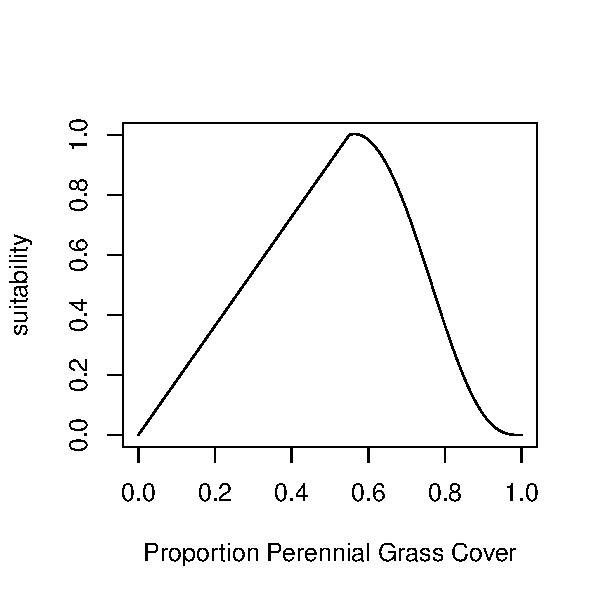
\includegraphics[width=\maxwidth]{figure/Sally-Dan_Grass_Cover_p} 
\end{knitrout}

\subsubsection{Annual}
\begin{knitrout}
\definecolor{shadecolor}{rgb}{0.969, 0.969, 0.969}\color{fgcolor}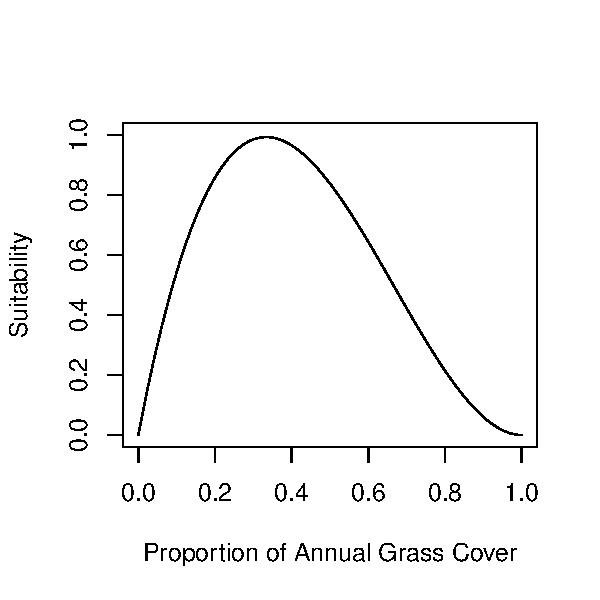
\includegraphics[width=\maxwidth]{figure/Sally-Dan_Grass_Cover_a} 
\end{knitrout}

\subsection{Grass Height}
\subsubsection{Dan Cohan}
\begin{knitrout}
\definecolor{shadecolor}{rgb}{0.969, 0.969, 0.969}\color{fgcolor}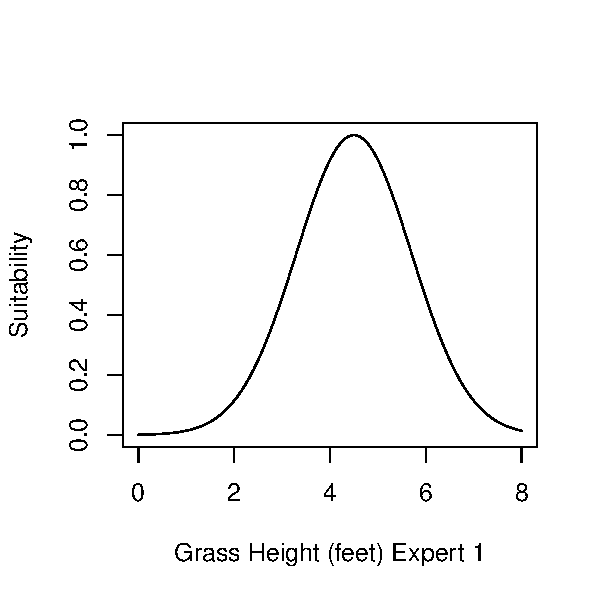
\includegraphics[width=\maxwidth]{figure/Dan_Grass_Height} 
\end{knitrout}

\subsubsection{Sally Gall}
\paragraph{Grass Height for Cover}
\begin{knitrout}
\definecolor{shadecolor}{rgb}{0.969, 0.969, 0.969}\color{fgcolor}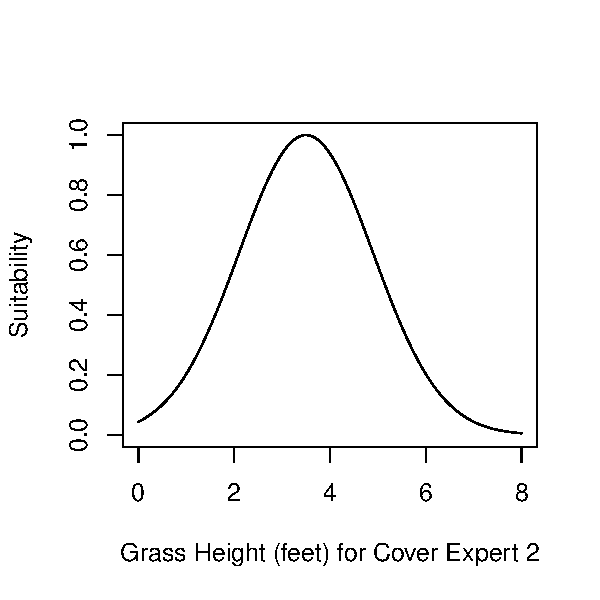
\includegraphics[width=\maxwidth]{figure/SAlly_Grass_Height_cover} 
\end{knitrout}

\paragraph{Grass Height for Nesting}
\begin{knitrout}
\definecolor{shadecolor}{rgb}{0.969, 0.969, 0.969}\color{fgcolor}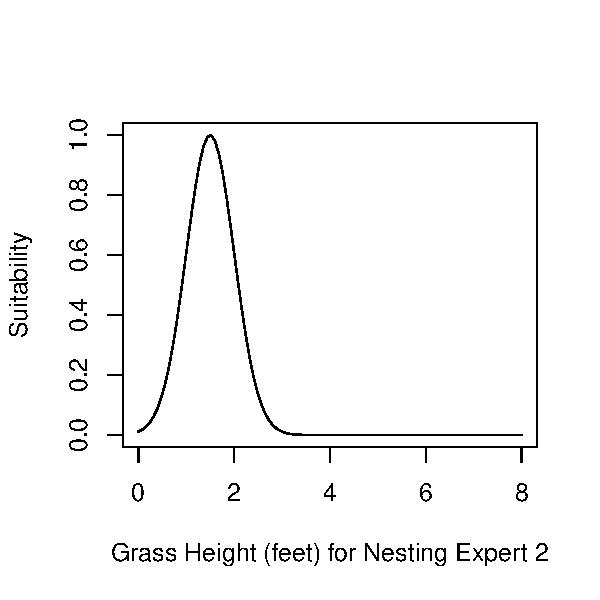
\includegraphics[width=\maxwidth]{figure/SAlly_Grass_Height_Nesting} 
\end{knitrout}

\subsection{Tree Cover}
\subsubsection{Uplands}
\begin{knitrout}
\definecolor{shadecolor}{rgb}{0.969, 0.969, 0.969}\color{fgcolor}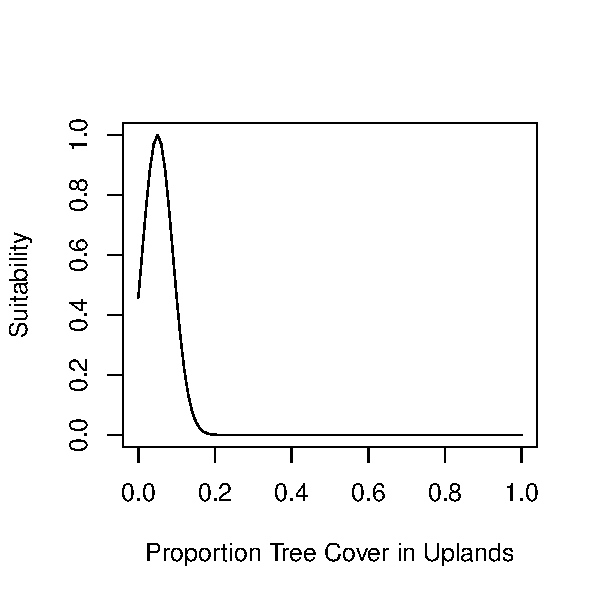
\includegraphics[width=\maxwidth]{figure/Sally-Dan_Tree_Cover_up} 
\end{knitrout}

\subsubsection{Arroyos}
\begin{knitrout}
\definecolor{shadecolor}{rgb}{0.969, 0.969, 0.969}\color{fgcolor}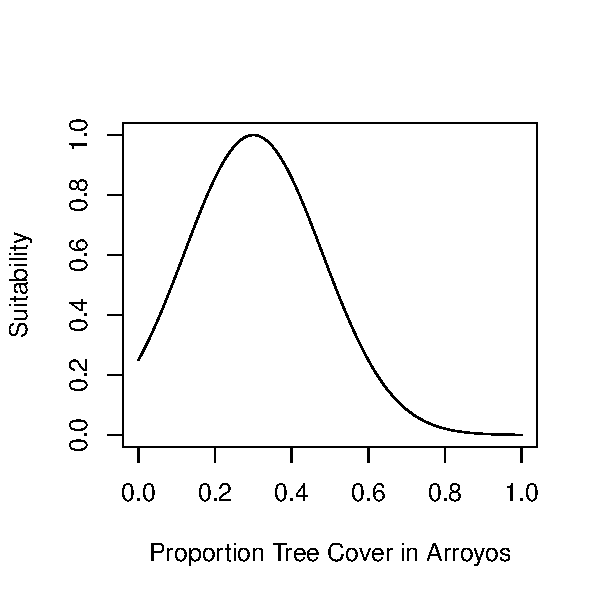
\includegraphics[width=\maxwidth]{figure/Sally-Dan_Tree_Cover_arroyo} 
\end{knitrout}

\subsection{Bare Ground}
\begin{knitrout}
\definecolor{shadecolor}{rgb}{0.969, 0.969, 0.969}\color{fgcolor}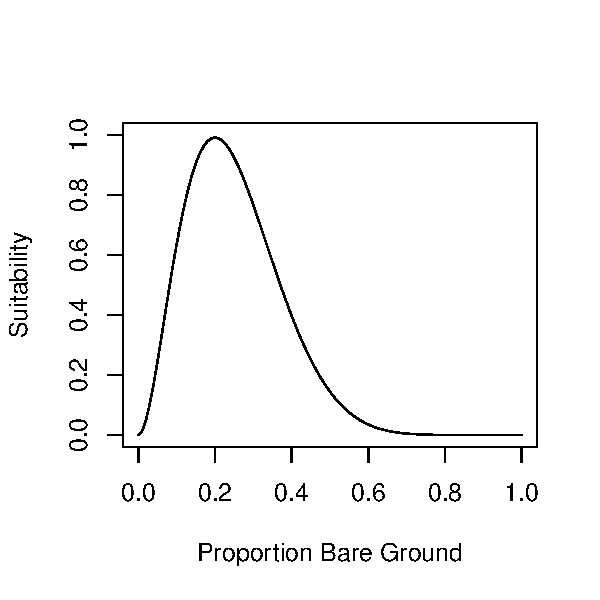
\includegraphics[width=\maxwidth]{figure/Sally-Dan_Bare_Ground} 
\end{knitrout}




\section{Roy Tomlinson}
\subsection{Forb Diveristy}
\begin{knitrout}
\definecolor{shadecolor}{rgb}{0.969, 0.969, 0.969}\color{fgcolor}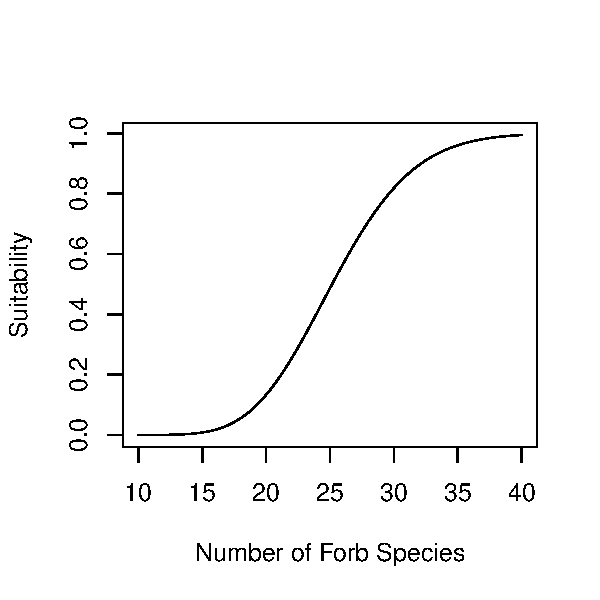
\includegraphics[width=\maxwidth]{figure/Roy_FD} 
\end{knitrout}

\subsection{Grass Diversity}
\begin{knitrout}
\definecolor{shadecolor}{rgb}{0.969, 0.969, 0.969}\color{fgcolor}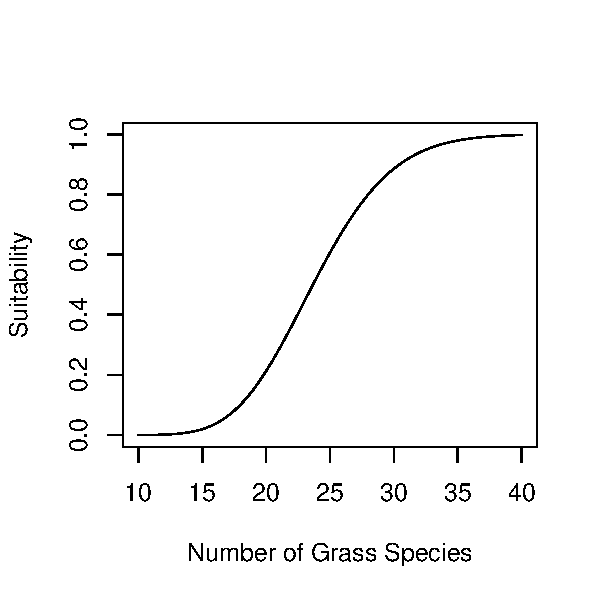
\includegraphics[width=\maxwidth]{figure/Grass_Diversity_Roy} 
\end{knitrout}

\subsection{Forb Height}
\begin{knitrout}
\definecolor{shadecolor}{rgb}{0.969, 0.969, 0.969}\color{fgcolor}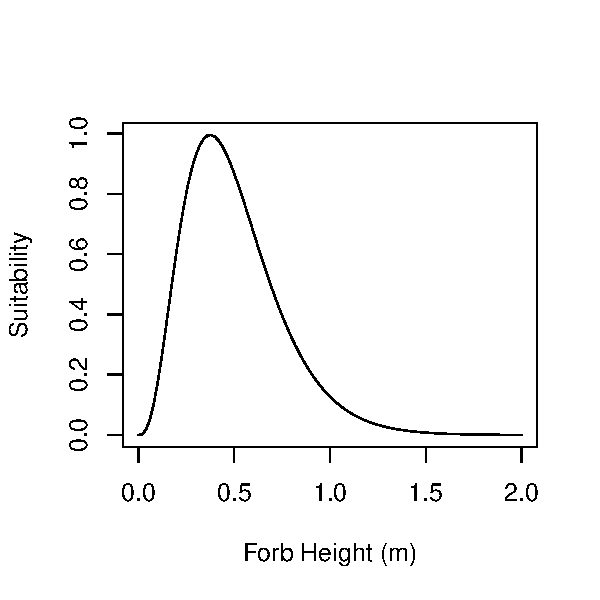
\includegraphics[width=\maxwidth]{figure/Roy_FH} 
\end{knitrout}

\subsection{Grass Height}
\begin{knitrout}
\definecolor{shadecolor}{rgb}{0.969, 0.969, 0.969}\color{fgcolor}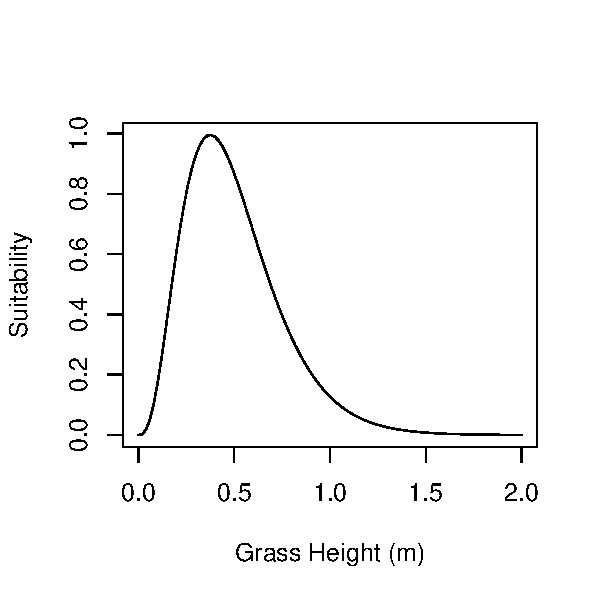
\includegraphics[width=\maxwidth]{figure/Roy_GH} 
\end{knitrout}

\subsection{Tree/Shrub Cover}
\subsubsection{Summer}
\begin{knitrout}
\definecolor{shadecolor}{rgb}{0.969, 0.969, 0.969}\color{fgcolor}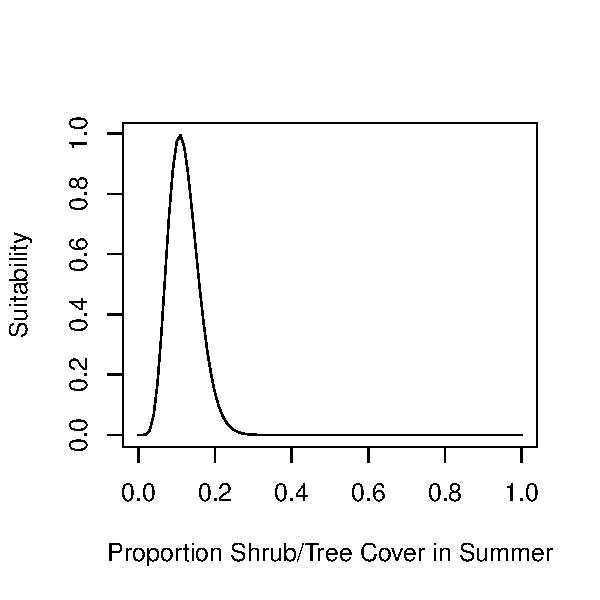
\includegraphics[width=\maxwidth]{figure/Shrub_Cover_Roy_Summer} 
\end{knitrout}

\subsubsection{Winter}
\begin{knitrout}
\definecolor{shadecolor}{rgb}{0.969, 0.969, 0.969}\color{fgcolor}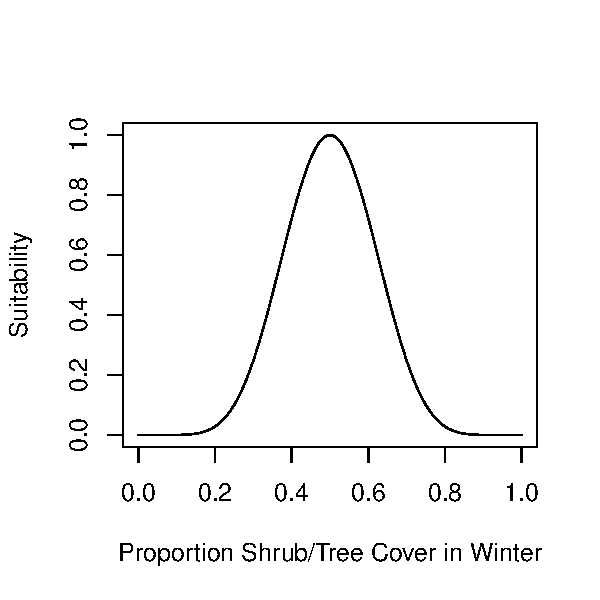
\includegraphics[width=\maxwidth]{figure/Shrub_Cover_Roy_Winter} 
\end{knitrout}

\subsection{Grass Cover}
\begin{knitrout}
\definecolor{shadecolor}{rgb}{0.969, 0.969, 0.969}\color{fgcolor}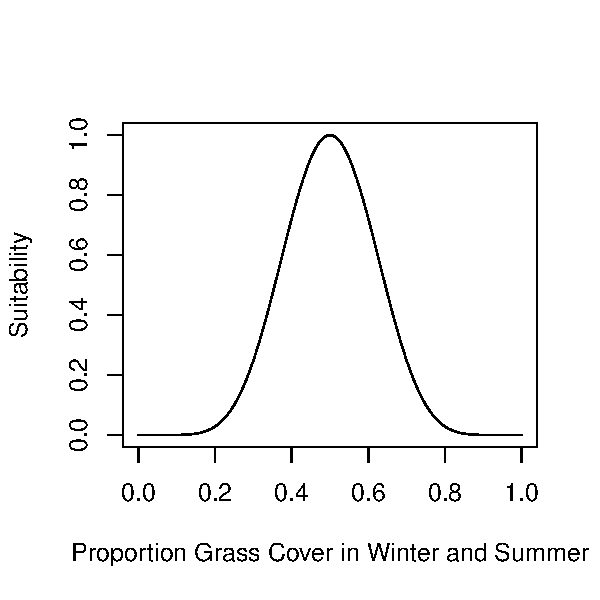
\includegraphics[width=\maxwidth]{figure/Grass_Cover_Roy} 
\end{knitrout}

\subsection{Forb Cover}
\subsubsection{Summer}
\begin{knitrout}
\definecolor{shadecolor}{rgb}{0.969, 0.969, 0.969}\color{fgcolor}\includegraphics[width=\maxwidth]{figure/Forb_Cover_Roy_Sum} 
\end{knitrout}

\subsubsection{Winter}
\begin{knitrout}
\definecolor{shadecolor}{rgb}{0.969, 0.969, 0.969}\color{fgcolor}\includegraphics[width=\maxwidth]{figure/Forb_Cover_Roy_Win} 
\end{knitrout}

\subsection{Bare Ground}
\begin{knitrout}
\definecolor{shadecolor}{rgb}{0.969, 0.969, 0.969}\color{fgcolor}\includegraphics[width=\maxwidth]{figure/Bare_Ground_Roy} 
\end{knitrout}

\end{document}
